\documentclass{beamer}

% Required packages
\usepackage{amsmath}
\usepackage{graphicx}
\usepackage{xcolor}
\usepackage{siunitx}

% Define custom colors for Star Trek DS9 theme
\definecolor{ds9blue}{RGB}{25,25,112}  % Midnight Blue
\definecolor{ds9gold}{RGB}{218,165,32} % Goldenrod
\definecolor{ds9grey}{RGB}{105,105,105} % Dim Gray
\definecolor{ds9red}{RGB}{178,34,34}   % Firebrick

% Set theme
\usetheme{Madrid}

% Customize colors
\setbeamercolor{palette primary}{bg=ds9blue,fg=white}
\setbeamercolor{palette secondary}{bg=ds9grey,fg=white}
\setbeamercolor{palette tertiary}{bg=ds9gold,fg=black}
\setbeamercolor{palette quaternary}{bg=ds9red,fg=white}
\setbeamercolor{structure}{fg=ds9blue}
\setbeamercolor{title}{fg=ds9gold}
\setbeamercolor{subtitle}{fg=ds9gold}
\setbeamercolor{frametitle}{bg=ds9blue,fg=white}
\setbeamercolor{block title}{bg=ds9blue,fg=white}
\setbeamercolor{block body}{bg=ds9grey!20,fg=black}

% Title page configuration
\title[Thermodynamics]{PHYS11 CH:12.1-12.4}
\subtitle{Laws of Thermodynamics and Applications}
\author[Mr. Gullo]{Mr. Gullo}
\date[March 2025]{March, 2025}
\institute{Physics Department}

\begin{document}

% Title slide
\begin{frame}
    \titlepage
\end{frame}

% Outline slide
\begin{frame}
    \frametitle{Overview}
    \tableofcontents
\end{frame}

% Learning objectives
\begin{frame}
    \frametitle{Learning Objectives}
    \begin{block}{By the end of this lesson, you will be able to:}
        \begin{itemize}
            \item Explain the concept of thermal equilibrium and the zeroth law
            \item Apply the first law of thermodynamics to calculate energy, work, and heat
            \item Understand entropy and the second law of thermodynamics
            \item Describe the working principles of heat engines, heat pumps, and refrigerators
            \item Calculate thermal efficiency of heat engines
            \item Relate thermodynamic principles to real-world applications
        \end{itemize}
    \end{block}
\end{frame}

\section{Zeroth Law of Thermodynamics}

\begin{frame}
    \frametitle{Thermal Equilibrium}
    \begin{columns}
        \column{0.6\textwidth}
        \begin{itemize}
            \item \textbf{Thermal Equilibrium:} Two systems have the same temperature
            \item \textbf{Thermal Contact:} Heat can transfer between objects
            \item Two objects in thermal contact will eventually reach thermal equilibrium
            \item At equilibrium, there is no net heat transfer
        \end{itemize}
        
        \column{0.4\textwidth}
        \begin{center}
            \begin{figure}
                \centering
                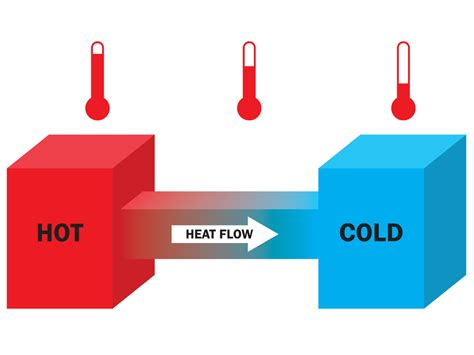
\includegraphics[width=0.75\linewidth]{phys11-thermo-thermal-equilibrium.jpg}
            \end{figure}
        \end{center}
    \end{columns}
    
    \begin{block}{Important Point}
        Thermal equilibrium occurs when two bodies are in contact with each other and can freely exchange energy.
    \end{block}
\end{frame}

\begin{frame}
    \frametitle{The Zeroth Law of Thermodynamics}
    \begin{block}{Zeroth Law Statement}
        If two systems, A and B, are in thermal equilibrium with each other, and B is in thermal equilibrium with a third system, C, then A is also in thermal equilibrium with C.
    \end{block}
    
    \begin{center}
        \begin{figure}
            \centering
            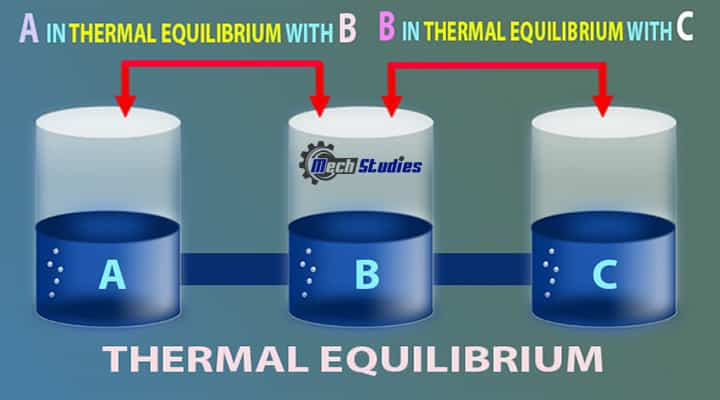
\includegraphics[width=0.5\linewidth]{phys11-thermo-zeroth-law.jpg}
        \end{figure}
    \end{center}
    
    \begin{exampleblock}{Mathematical Analogy}
        Similar to the transitive property in mathematics:
        
        If A = B and B = C, then A = C
    \end{exampleblock}
\end{frame}

\section{First Law of Thermodynamics}

\begin{frame}
    \frametitle{Pressure and Thermal Expansion}
    \begin{columns}
        \column{0.5\textwidth}
        \textbf{Pressure:}
        \begin{itemize}
            \item Force per unit area
            \begin{align*}
                P = \frac{F}{A}
            \end{align*}
            \item SI unit: Pascal (Pa) = N/m²
        \end{itemize}
        
        \column{0.5\textwidth}
        \textbf{Thermal Expansion:}
        \begin{itemize}
            \item Change in size due to temperature change
            \item Results from increased molecular motion
            \item Important in engineering and everyday applications (bridges, thermostats, etc.)
        \end{itemize}
    \end{columns}
    
    \begin{block}{Why does thermal expansion occur?}
        An increase in temperature causes intermolecular distances to increase as particles gain kinetic energy.
    \end{block}
\end{frame}

\begin{frame}
    \frametitle{Ideal Gas Law}
    \begin{alertblock}{Ideal Gas Law}
        \begin{align*}
            PV = NkT
        \end{align*}
        where:
        \begin{itemize}
            \item $P$ = pressure (Pa)
            \item $V$ = volume (m³)
            \item $N$ = number of particles
            \item $k$ = Boltzmann constant ($1.38 \times 10^{-23}$ J/K)
            \item $T$ = absolute temperature (K)
        \end{itemize}
    \end{alertblock}
    \end{frame}

\begin{frame}
    \begin{exampleblock}{Real vs. Ideal Gases}
        A real gas behaves most like an ideal gas at:
        \begin{itemize}
            \item High temperatures
            \item Low pressures
        \end{itemize}
        Under these conditions, particle interactions become negligible.
    \end{exampleblock}
\end{frame}

\begin{frame}
    \frametitle{Energy Transfer: Heat and Work}
    \begin{block}{Two Methods of Energy Transfer}
        \begin{itemize}
            \item \textbf{Heat (Q):} Energy transferred solely due to a temperature difference
            \item \textbf{Work (W):} Energy transfer that doesn't rely on temperature difference
        \end{itemize}
    \end{block}
    
    \begin{exampleblock}{Pressure-Volume Work}
        \begin{align*}
            W = P\Delta V
        \end{align*}
        
        \begin{itemize}
            \item Work is done \textit{by} a system when it \textit{expands} ($\Delta V > 0$)
            \item Work is done \textit{on} a system when it is \textit{compressed} ($\Delta V < 0$)
        \end{itemize}
    \end{exampleblock}
    
    \begin{center}
        \alert{[Diagram showing work done by/on a gas in a piston]}
    \end{center}
\end{frame}

\begin{frame}
\begin{figure}
    \centering
    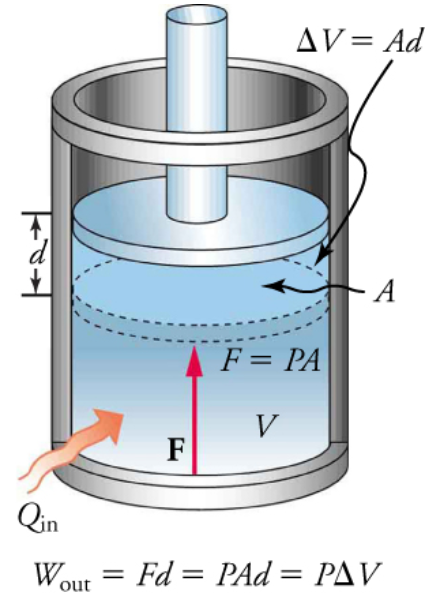
\includegraphics[width=0.4\linewidth]{phys11-thermo-work-done-by-gas-piston.png}
\end{figure}
\end{frame}

\begin{frame}
    \frametitle{First Law of Thermodynamics}
    \begin{alertblock}{First Law Statement}
        The change in internal energy of a system equals the net heat transferred into the system minus the net work done by the system.
        
        \begin{align*}
            \Delta U = Q - W
        \end{align*}
        
        where:
        \begin{itemize}
            \item $\Delta U$ = change in internal energy
            \item $Q$ = net heat transferred into the system
            \item $W$ = net work done by the system
        \end{itemize}
    \end{alertblock}
    \end{frame}

\begin{frame}
    \begin{block}{Key Insights}
        \begin{itemize}
            \item The first law is an application of the conservation of energy
            \item Internal energy ($U$) depends only on the state of the system
            \item $Q$ and $W$ represent energy in transit; only $\Delta U$ represents stored energy
        \end{itemize}
    \end{block}
\end{frame}

\section{Second Law of Thermodynamics}

\begin{frame}
    \frametitle{Entropy}
    \begin{columns}
        \column{0.6\textwidth}
        \begin{block}{What is Entropy?}
            \begin{itemize}
                \item A measure of a system's disorder
                \item The reduced availability of energy to do work
                \item SI unit: joules per kelvin (J/K)
            \end{itemize}
        \end{block}
        
        \column{0.4\textwidth}
        \begin{center}
            \begin{figure}
                \centering
                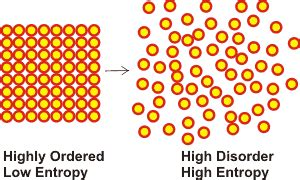
\includegraphics[width=0.8\linewidth]{phys11-thermo-entropy-disorder.jpg}
            \end{figure}
        \end{center}
    \end{columns}
    
    \begin{exampleblock}{Change in Entropy}
        \begin{align*}
            \Delta S = \frac{Q}{T}
        \end{align*}
        where:
        \begin{itemize}
            \item $\Delta S$ = change in entropy
            \item $Q$ = heat transferred
            \item $T$ = absolute temperature
        \end{itemize}
    \end{exampleblock}
\end{frame}

\begin{frame}
    \frametitle{Second Law of Thermodynamics}
    \begin{alertblock}{Second Law Statement}
        For any spontaneous process, the total entropy of a system either increases or remains constant; it never decreases.
    \end{alertblock}
    
    \begin{block}{Implications of the Second Law}
        \begin{itemize}
            \item Heat flows spontaneously from higher to lower temperature, never the reverse
            \item Energy tends to disperse from concentrated to dispersed states
            \item Perfect heat engines (100\% efficiency) are impossible
            \item All natural processes are irreversible
        \end{itemize}
    \end{block}
    
    \begin{exampleblock}{Everyday Examples}
        \begin{itemize}
            \item Air freshener molecules dispersing in a room
            \item Ice melting in water
            \item Spreading of salt in water
        \end{itemize}
    \end{exampleblock}
\end{frame}

\section{Applications of Thermodynamics}

\begin{frame}
    \frametitle{Heat Engines}
    \begin{columns}
        \column{0.55\textwidth}
        \begin{itemize}
            \item \textbf{Heat Engine:} Device that converts thermal energy to mechanical work
            \item Uses temperature difference between hot and cold reservoirs
            \item Works through a cyclic process
            \item Examples: steam engines, internal combustion engines, gas turbines
        \end{itemize}
        
        \column{0.45\textwidth}
        \begin{center}
            \begin{figure}
                \centering
                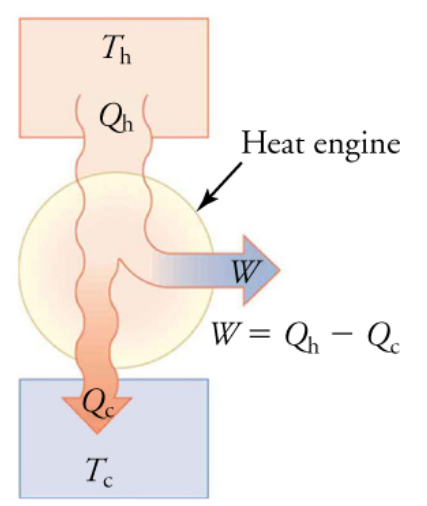
\includegraphics[width=0.7\linewidth]{phys11-thermo-heat-engine-diagram.png}
            \end{figure}
        \end{center}
    \end{columns}
    
    \begin{block}{Cyclic Process}
        A process that returns to its original state at the end of every cycle, so that the change in internal energy is zero ($\Delta U = 0$).
    \end{block}
\end{frame}

\begin{frame}
    \frametitle{Thermal Efficiency}
    \begin{alertblock}{Thermal Efficiency Formula}
        \begin{align*}
            \text{eff} = \frac{W}{Q_h} = \frac{Q_h - Q_c}{Q_h} = 1 - \frac{Q_c}{Q_h}
        \end{align*}
        where:
        \begin{itemize}
            \item eff = thermal efficiency
            \item $W$ = work output
            \item $Q_h$ = heat input from hot reservoir
            \item $Q_c$ = heat output to cold reservoir
        \end{itemize}
    \end{alertblock}
    \end{frame}

\begin{frame}
    \begin{block}{Important Points}
        \begin{itemize}
            \item Efficiency is always less than 100\%
            \item Some heat is always lost to the environment
            \item Efficiency would be 100\% only if $Q_c = 0$ (impossible due to the second law)
            \item For a cyclical process, work output $W = Q_h - Q_c$
        \end{itemize}
    \end{block}
\end{frame}

\begin{frame}
    \frametitle{Heat Pumps and Refrigerators}
    \begin{columns}
        \column{0.5\textwidth}
        \textbf{Heat Pump:}
        \begin{itemize}
            \item Transfers heat from cold to hot environment
            \item Requires work input
            \item Used for heating buildings
            \item Energy efficient compared to direct heating
        \end{itemize}
        
        \column{0.5\textwidth}
        \textbf{Refrigerator:}
        \begin{itemize}
            \item A type of heat pump
            \item Removes heat from inside to outside
            \item Components: compressor, condenser, expansion valve, evaporator
        \end{itemize}
    \end{columns}
    
    \begin{block}{Advantage of Heat Pumps}
        A heat pump supplies energy by heat from the cold, outside air and also from the energy generated by the work done.
    \end{block}
    
    \begin{center}
        \alert{[Diagram showing heat pump/refrigerator cycle]}
    \end{center}
\end{frame}


\begin{frame}
\begin{figure}
    \centering
    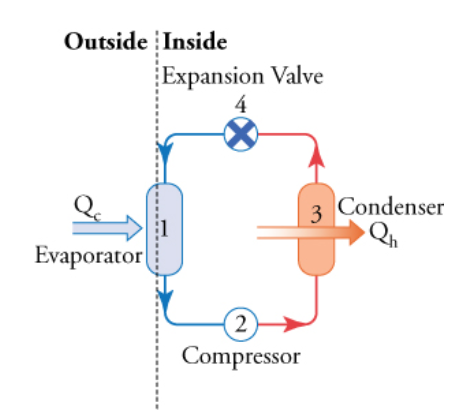
\includegraphics[width=0.75\linewidth]{phys11-thermo-heat-pump-refrigerator-cycle.png}
\end{figure}
\end{frame}
\section{Examples and Applications}

\begin{frame}
    \frametitle{"I do" Example}
    \begin{block}{Problem}
        Some amount of energy is transferred by heat into a system. The net work done by the system is 50 J, while the increase in its internal energy is 30 J. What is the amount of net heat?
    \end{block}
    \end{frame}

\begin{frame}
    \begin{exampleblock}{Solution}
        \begin{enumerate}
            \item Use the first law of thermodynamics: $\Delta U = Q - W$
            \item Given information:
            \begin{itemize}
                \item $\Delta U = 30$ J (increase in internal energy)
                \item $W = 50$ J (net work done by the system)
            \end{itemize}
            
            \item Rearrange the equation to solve for $Q$:
            \begin{align*}
                Q &= \Delta U + W\\
                &= 30 \text{ J} + 50 \text{ J}\\
                &= 80 \text{ J}
            \end{align*}
            
            \item Therefore, the amount of net heat transferred to the system is 80 J.
        \end{enumerate}
    \end{exampleblock}
\end{frame}

\begin{frame}
    \frametitle{"We do" Example}
    \begin{block}{Problem}
        Assume 310 J of heat enter a system, after which the system does 120 J of work. What is the change in its internal energy? Would this amount change if the energy transferred by heat were added after the work was done instead of before?
    \end{block}
    \pause
    \begin{exampleblock}{Solution Steps}
        \begin{enumerate}
            \item Apply the first law of thermodynamics: $\Delta U = Q - W$
            \item Given information:
            \begin{itemize}
                \item $Q = 310$ J (heat entering the system)
                \item $W = 120$ J (work done by the system)
            \end{itemize}
            
            \item Calculate the change in internal energy:
            \begin{align*}
                \Delta U &= Q - W \\
                &= 310 \text{ J} - 120 \text{ J} \\
                &= 190 \text{ J}
            \end{align*}
             \end{enumerate}
    \end{exampleblock}
    
    Let's work through this together!
\end{frame}

\begin{frame}
    \frametitle{"You do" Example}
    \begin{block}{Problem}
        A coal power station functions at 40.0 percent efficiency. What is the amount of work it does if it takes in 4.00×10⁶ J by heat?
    \end{block}
    \pause
    \begin{alertblock}{Hints}
        \begin{itemize}
            \item Use the thermal efficiency formula: $\text{eff} = \frac{W}{Q_h}$
            \item Efficiency is given as a percentage (40.0\%)
            \item Heat input ($Q_h$) is 4.00×10⁶ J
        \end{itemize}
    \end{alertblock}
    
    Take some time to work this out. Then we'll discuss the solution.
    
    \pause
    
    \begin{exampleblock}{Answer}
        The work done by the power station is 1.60×10⁶ J.
    \end{exampleblock}
\end{frame}

\section{Summary}

\begin{frame}
    \frametitle{Key Equations}
    \begin{columns}
        \column{0.5\textwidth}
        \textbf{First Law of Thermodynamics:}
        \begin{align*}
            \Delta U &= Q - W \\
            PV &= NkT \\
            P &= \frac{F}{A} \\
            W &= P\Delta V
        \end{align*}
        
        \column{0.5\textwidth}
        \textbf{Second Law and Applications:}
        \begin{align*}
            \Delta S &= \frac{Q}{T} \\
            \text{eff} &= \frac{W}{Q_h} \\
            W &= Q_h - Q_c
        \end{align*}
    \end{columns}
\end{frame}

\begin{frame}
    \frametitle{Laws of Thermodynamics Summary}
    \begin{block}{Zeroth Law}
        If two systems are each in thermal equilibrium with a third system, they are in thermal equilibrium with each other.
    \end{block}
    
    \begin{block}{First Law}
        Energy can be transferred and transformed, but it cannot be created or destroyed.
        
        $\Delta U = Q - W$
    \end{block}
    
    \begin{block}{Second Law}
        For any spontaneous process, the total entropy of a system either increases or remains constant; it never decreases.
    \end{block}
    
    \begin{block}{Practical Applications}
        Heat engines, power plants, refrigerators, heat pumps, and many industrial processes rely on thermodynamic principles.
    \end{block}
\end{frame}

\begin{frame}
    \frametitle{Thank You!}
    \begin{center}
        \Huge{Questions?}
        
        \vspace{1cm}
        \normalsize
        Remember to review the key laws and concepts for the upcoming quiz!
    \end{center}
\end{frame}

\end{document}